\chapter[Degree One]{Degree One: Dirichlet Characters,\\ Hecke Characters and Complex Multiplication}\label{ch:gl1}

Reciprocity for $\GL_1$ is a theorem. Over $\Q$ it is the theorem of Kronecker and Weber, that every one dimensional representation of $\Gal(\overline\Q/\Q)$ is a Dirichlet character; over a number field $K$ it is Artin's reciprocity law, that the one dimensional representations are the characters of ray class groups, which Hecke extended to characters of infinite order with entire $L$ functions. Everything the book does for $\GL_2$ under hypotheses it can do for $\GL_1$ without them, and this chapter does it: Dirichlet's theorem on primes in progressions becomes a Dirichlet process on the classes mod $q$, with Mertens constants computed from $L(1,\chi)$ and with Landau's theorem on integers without prime factors in a class as the atom at zero of Chapter~\ref{ch:pd}; Hecke's theorem on the angles of Gaussian primes becomes a Dirichlet process on the circle; and the Thorin measure of a degree one $L$ function is checked against its zeros to $2\cdot10^{-8}$.

The chapter then treats the one case of $\GL_2$ reciprocity that reduces to $\GL_1$, complex multiplication. Deuring's theorem says that the $L$ function of an elliptic curve with complex multiplication by $K$ is the $L$ function of a Hecke character of $K$, so that a degree two Euler product over $\Q$ is a degree one Euler product over $K$. The Frobenius angles of such a curve are the arguments of Gaussian integers, their law is half uniform and half an atom, and the Rankin Selberg subordinator of Chapter~\ref{ch:recip} has an exact property that no curve without complex multiplication shares: seen from $K$ it is the sum of two independent copies of itself seen from $\Q$, so that its Gamma shape is $2$ rather than $1$. This is the Gamma shape test of Theorem~\ref{thm:recipgamma} detecting complex multiplication, and it is proved, not conjectured. In the logic of the book the chapter belongs early, after the Galois representations of Chapter~\ref{ch:03} and before the equidistribution of Part~II; it is placed here, after Chapter~\ref{ch:pd}, because it is the one place where the reader can see every object of Chapters~\ref{ch:recip} to \ref{ch:pd} with nothing left to prove.

\section{Dirichlet characters and the random integer mod \texorpdfstring{$q$}{q}}\label{sec:gl1dirichlet}

Fix $q\ge3$. The cyclotomic field $\Q(\zeta_q)$ has Galois group $(\Z/q\Z)^\times$, and the Frobenius class of a prime $p\nmid q$ is the residue of $p$ modulo $q$. Chebotarev's theorem for this field is Dirichlet's theorem: each residue class $a$ prime to $q$ receives primes with density $1/\varphi(q)$. The Haar measure of Chapter~\ref{ch:recip} is counting measure on $(\Z/q\Z)^\times$ divided by $\varphi(q)$, and the characters of the group are the Dirichlet characters modulo $q$.

Let $N_\sigma$ be the zeta distributed random integer of Chapter~\ref{ch:recip}, $\Prob(N_\sigma=n)=n^{-\sigma}/\zeta(\sigma)$, with the primes dividing $q$ removed as in Section~\ref{sec:pdprogress}, and colour each prime factor by its residue class. Everything in Chapters~\ref{ch:recip} and \ref{ch:pd} applies with $G=(\Z/q\Z)^\times$ and every class of size one.

\begin{theorem}[Dirichlet's theorem in law]\label{thm:gl1dirichlet}
Let $q\ge3$ and $\sigma\downarrow1$.
\begin{enumerate}
\item[(i)] The vector of shares $(P_\sigma(a))_{a\in(\Z/q\Z)^\times}$, $P_\sigma(a)$ the fraction of $\log N_\sigma$ carried by the prime factors congruent to $a$, converges in law to the Dirichlet law with all parameters $1/\varphi(q)$; the labelled factorisation converges to Ferguson's Dirichlet process with base measure the uniform law on $(\Z/q\Z)^\times$.
\item[(ii)] For every $a$ the probability that $N_\sigma$ has no prime factor congruent to $a$ is $e^{-h_a(1)}(\sigma-1)^{1/\varphi(q)}(1+o(1))$, where $e^{h_a(1)}$ is the regular part at $s=1$ of $\prod_{p\equiv a}(1-p^{-s})^{-1}(s-1)^{1/\varphi(q)}$.
\item[(iii)] (Mertens for progressions.) $\sum_{p\le x,\,p\equiv a}p^{-1}=\varphi(q)^{-1}\log\log x+M(q,a)+o(1)$ with
\[
M(q,a)=\frac1{\varphi(q)}\Bigl[M-\sum_{p\mid q}\frac1p+\sum_{\chi\ne\chi_0}\bar\chi(a)S(\chi)\Bigr],
\]
where $S(\chi)=\log L(1,\chi)-\sum_{k\ge2}\sum_p\chi(p)^k(kp^{k})^{-1}$,
$M=0.2614972\ldots$ the Mertens constant, and
\[
h_a(1)=M(q,a)-\frac{\gamma}{\varphi(q)}+\sum_{k\ge2}\sum_{p\equiv a}\frac1{kp^k}.
\]
\end{enumerate}
\end{theorem}

\begin{proof}
(i) is Theorem~\ref{thm:pddirichlet} with $\mu$ uniform on $(\Z/q\Z)^\times$, the equidistribution hypothesis being Dirichlet's theorem. (ii) is Theorem~\ref{thm:pdrate} with $\delta(C)=1/\varphi(q)$. (iii) is Theorem~\ref{thm:pdmertensL} written out: by orthogonality of characters,
\[
\sum_{p\equiv a}p^{-s}=\frac1{\varphi(q)}\sum_\chi\bar\chi(a)\sum_{p\nmid q}\chi(p)p^{-s},
\]
and $\sum_p\chi(p)p^{-s}=\log L(s,\chi)-\sum_{k\ge2}\sum_p\chi(p)^k(kp^{ks})^{-1}$ for $\operatorname{Re}s>1$, continuous up to $s=1$ for $\chi\ne\chi_0$ since $L(1,\chi)\ne0$. The principal character contributes $\sum_{p\le x}p^{-1}-\sum_{p\mid q}p^{-1}$ and Mertens' theorem. The formula for $h_a(1)$ compares two products. By (iii),
\[
\prod_{p\equiv a,\,p\le x}\Bigl(1-\frac1p\Bigr)^{-1}=\exp\Bigl(\frac{\log\log x}{\varphi(q)}+M(q,a)+\sum_{k\ge2}\sum_{p\equiv a}\frac1{kp^k}+o(1)\Bigr),
\]
while $\prod_{p\equiv a}(1-p^{-s})^{-1}\sim e^{h_a(1)}(s-1)^{-1/\varphi(q)}$ by definition. Mertens' theorem $\prod_{p\le x}(1-p^{-1})^{-1}\sim e^\gamma\log x$ and $\zeta(s)\sim(s-1)^{-1}$ relate the two scales, and the class carries the fraction $1/\varphi(q)$ of the exponent, which is the factor $e^{-\gamma/\varphi(q)}$, as in the proof of Theorem~\ref{thm:pdmertensL}.
\end{proof}

For $q=4$ the only nonprincipal character is $\chi_4$ with $L(1,\chi_4)=\pi/4$, and
\[
M(4,1)=-0.286742,\qquad M(4,3)=0.048239,
\]
against the sums over the primes below $10^7$, which give $-0.286728$ and $0.048235$, the difference being the tail beyond $10^7$. The atoms at zero are
\[
\Prob(\text{no factor }\equiv3)\sim e^{-h_3(1)}\sqrt{\sigma-1},\qquad e^{-2h_3(1)}=2L(1,\chi_4)\prod_{p\equiv3\,(4)}(1-p^{-2}),
\]
with $e^{-h_3(1)}=1.159643$
and $e^{-h_1(1)}=2/e^{-h_3(1)}=1.724668$, since the two classes together exhaust the odd primes and $\prod_{p\text{ odd}}(1-p^{-\sigma})\sim2(\sigma-1)$. The exact values $\prod_{p\equiv3}(1-p^{-\sigma})/\sqrt{\sigma-1}$ are $1.1255$, $1.1563$, $1.1593$, $1.1596$ at $\sigma-1=10^{-1},\dots,10^{-4}$ (Figure~\ref{fig:gl1landau}, right). The closed forms come from $\zeta^{(2)}(s)L(s,\chi_4)=\prod_{p\equiv1}(1-p^{-s})^{-2}\prod_{p\equiv3}(1-p^{-2s})^{-1}$ and its companion with $L$ in the denominator, which express each partial Euler product through $\zeta$, $L(s,\chi_4)$ and a rapidly convergent product over squares.

\begin{figure}[t]
\centering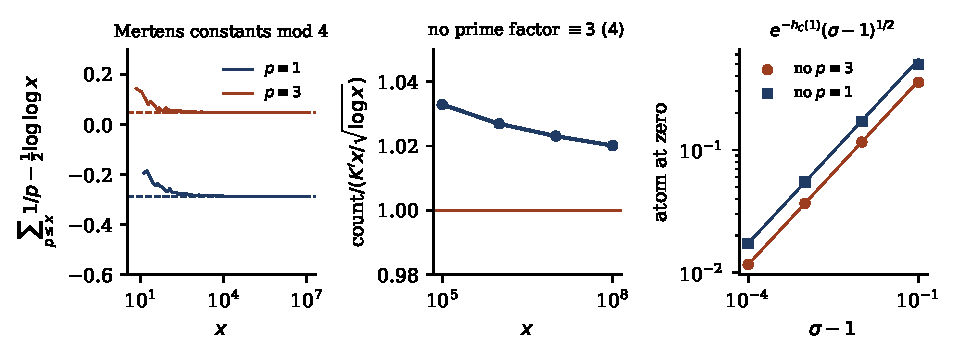
\includegraphics[width=\textwidth]{figs/gl1_landau.pdf}
\caption{Dirichlet's theorem in law for $q=4$. Left: the running sums $\sum_{p\le x,\,p\equiv a}p^{-1}-\frac12\log\log x$ for the two classes, converging to the Mertens constants $M(4,1)=-0.2867$ and $M(4,3)=0.0482$ computed from $L(1,\chi_4)$ (dashed). Middle: the number of integers below $x$ with no prime factor congruent to $3$ modulo $4$, divided by $K'x/\sqrt{\log x}$ with $K'=0.654259$; the excess decays like $1/\log x$. Right: the probability that the zeta distributed integer has no prime factor in a class modulo $4$, against $e^{-h_C(1)}(\sigma-1)^{1/2}$.}\label{fig:gl1landau}
\end{figure}

The atom at zero has a classical counterpart for the uniform integer, due to Landau, which Theorem~\ref{thm:pdrate} identifies with its constant.

\begin{theorem}[Landau's theorem with Wirsing's constant]\label{thm:gl1landau}
The number of $n\le x$ all of whose odd prime factors are congruent to $1$ modulo $4$ is
\[
K'\frac{x}{\sqrt{\log x}}(1+o(1)),\qquad K'=\Bigl(\tfrac12\prod_{p\equiv3\,(4)}(1-p^{-2})\Bigr)^{1/2}=0.654259\ldots
\]
By comparison the number of $n\le x$ that are sums of two squares is $Kx/\sqrt{\log x}$ with the Landau Ramanujan constant $K=(2\prod_{p\equiv3}(1-p^{-2}))^{-1/2}=0.764224\ldots$, and $K'/K=\prod_{p\equiv3\,(4)}(1-p^{-2})=0.856109$, the probability that an integer is not divisible by the square of any prime congruent to $3$ modulo $4$.
\end{theorem}

\begin{proof}
The generating Dirichlet series is $F(s)=(1-2^{-s})^{-1}\prod_{p\equiv1}(1-p^{-s})^{-1}$ and, by the identity above, $F(s)^2=(1-2^{-s})^{-1}\zeta(s)L(s,\chi_4)\prod_{p\equiv3}(1-p^{-2s})$, so $F(s)\sim C(s-1)^{-1/2}$ with $C^2=2L(1,\chi_4)\prod_{p\equiv3}(1-p^{-2})=\frac\pi2\prod_{p\equiv3}(1-p^{-2})$. The coefficients of $F$ are the indicator of the set, a multiplicative function with values in $\{0,1\}$ whose sum over primes $p\le x$ is $\frac12x/\log x$, so Wirsing's theorem \cite{wirsing1961}, in the form used in Theorem~\ref{thm:pdrate}, gives the count $Cx(\log x)^{-1/2}/\Gamma(\frac12)$, and $C/\sqrt\pi=K'$. In the notation of Theorem~\ref{thm:pdrate}, $K'=e^{-h_3(1)}/\Gamma(\frac12)$ with $e^{-h_3(1)}=1.159643$ as computed above, since the integers counted are exactly those with no prime factor in the class of $3$. The sums of two squares have generating series $\bigl(\zeta(s)L(s,\chi_4)(1-2^{-s})^{-1}\prod_{p\equiv3}(1-p^{-2s})^{-1}\bigr)^{1/2}$, which gives $K$ \cite{landau1908}.
\end{proof}

A sieve to $10^8$ gives counts $19915$, $180751$, $1667197$ and $15550333$ at $x=10^5,\dots,10^8$, which are $1.033$, $1.027$, $1.023$ and $1.020$ times $K'x/\sqrt{\log x}$ (Figure~\ref{fig:gl1landau}, left); the excess is the secondary term $c/\log x$ of the Selberg Delange expansion, with $c\approx0.37$.

\section{Reciprocity for \texorpdfstring{$\GL_1$}{GL1}: class field theory as measurability}\label{sec:gl1cft}

The statements of reciprocity in degree one are these.

\begin{theorem}[Kronecker, Weber; Artin; Hecke]\label{thm:gl1cft}
\begin{enumerate}
\item[(i)] Every continuous one dimensional representation of $\Gal(\overline\Q/\Q)$ factors through $\Gal(\Q(\zeta_q)/\Q)$ for some $q$, hence is a Dirichlet character.
\item[(ii)] For a number field $K$ and a modulus $\mathfrak f$, the Artin map $\mathfrak p\mapsto\Frob_{\mathfrak p}$ induces an isomorphism from the ray class group modulo $\mathfrak f$ onto $\Gal(K_{\mathfrak f}/K)$, $K_{\mathfrak f}$ the ray class field, and every abelian extension of $K$ lies in some $K_{\mathfrak f}$. Hence the one dimensional representations of $\Gal(\overline K/K)$ are the characters of ray class groups.
\item[(iii)] A Hecke character of $K$ is a character $\psi$ of the group of fractional ideals prime to $\mathfrak f$ for which there is a continuous character $\psi_\infty$ of $(K\otimes\R)^\times$ with $\psi((\alpha))=\psi_\infty(\alpha)^{-1}$, or $\psi_\infty(\alpha)$ in the convention of this book, for $\alpha\equiv1$ modulo $\mathfrak f$. Its $L$ function $L(s,\psi)=\prod_{\mathfrak p\nmid\mathfrak f}(1-\psi(\mathfrak p)N\mathfrak p^{-s})^{-1}$ has meromorphic continuation and a functional equation, and is entire unless $\psi$ is a power of the norm.
\end{enumerate}
\end{theorem}

The characters of finite order in (iii) are the ray class characters of (ii); the characters of infinite order, Hecke's Gr\"ossencharaktere \cite{hecke1920}, are the automorphic representations of $\GL_1(\A_K)$ that are not Artin representations (the algebraic ones among them are $\ell$ adic characters of $\Gal(\overline K/K)$, which is how $\psi$ appears in Section~\ref{sec:gl1cm}), and they are the subject of Sections~\ref{sec:gl1hecke} and \ref{sec:gl1cm}.

The probabilistic reading is Proposition~\ref{prop:recipcongruence}: a Frobenius random variable $p\mapsto\rho(\Frob_p)$ on the probability space of primes is measurable with respect to the congruence $\sigma$ algebra, the one generated by the events $\{p\equiv a\ (q)\}$, if and only if $\rho$ is abelian. Theorem~\ref{thm:gl1cft}(i) is the statement that for one dimensional $\rho$ this is always so. The Dirichlet process of Theorem~\ref{thm:gl1dirichlet} is the normalised Gamma process of Theorem~\ref{thm:recipgammaproc} seen through that $\sigma$ algebra, and its base measure is uniform because the Frobenius elements of an abelian extension of $\Q$ are equidistributed in the Galois group, which is Dirichlet's theorem again.

\section{Hecke characters of \texorpdfstring{$\Q(i)$}{Q(i)} and the angles of Gaussian primes}\label{sec:gl1hecke}

Let $K=\Q(i)$, with ring of integers $\Z[i]$, units $\{\pm1,\pm i\}$, and class number one. A prime $p\equiv1$ modulo $4$ splits as $p=\pi\bar\pi$ with $\pi=a+bi$, $p=a^2+b^2$; a prime $p\equiv3$ stays prime, with residue degree two; and $2=-i(1+i)^2$ ramifies. Among the four associates of $\pi$ exactly one is \emph{primary}, $\pi\equiv1$ modulo $(2+2i)$, which for $a+bi$ means $a$ odd, $b$ even and $a+b\equiv1$ modulo $4$; the primary generator is the one used by Gauss for biquadratic reciprocity. Both $\pi$ and $\bar\pi$ are primary. Write $\theta_p=|\arg\pi|\in[0,\pi]$, which is the same for both, and note that the argument of any generator is $\pm\theta_p$ plus a multiple of $\pi/2$, so $4\theta_p$ modulo $2\pi$ is well defined up to sign.

For $k\in\Z$ the function $\lambda_k((\alpha))=(\alpha/|\alpha|)^{4k}$ is well defined on all nonzero ideals, since the units are fourth roots of unity, and it is a Hecke character of $K$ with trivial conductor and infinity type $z\mapsto(z/|z|)^{4k}$. Its $L$ function $L(s,\lambda_k)$ is entire for $k\ne0$ and does not vanish on $\operatorname{Re}s=1$ (Hecke).

\begin{theorem}[Hecke \cite{hecke1920}]\label{thm:gl1hecke}
The angles $4\theta_p$, $p\equiv1$ modulo $4$, are equidistributed modulo $2\pi$: for every continuous $f$ on the circle, $\frac1{\pi_1(x)}\sum_{p\le x,\,p\equiv1}f(4\theta_p)\to\frac1{2\pi}\int_0^{2\pi}f$. More precisely the arguments of the primary Gaussian primes, both $\pi$ and $\bar\pi$ for each $p$, are equidistributed on the circle, so that $\theta_p$ is equidistributed on $[0,\pi]$.
\end{theorem}

\begin{proof}
By Weyl's criterion it suffices that $\sum_{p\le x,p\equiv1}e^{4ik\theta_p}=o(x/\log x)$ for $k\ne0$. The sum is $\sum_{N\mathfrak p\le x}\lambda_k(\mathfrak p)$ over the degree one primes of $K$, up to the $O(\sqrt x)$ primes of degree two, and the prime ideal theorem for $L(s,\lambda_k)$, that is the nonvanishing on $\operatorname{Re}s=1$ with the Wiener Ikehara theorem applied to $-L'/L$, gives $\sum_{N\mathfrak p\le x}\lambda_k(\mathfrak p)=o(x/\log x)$. For the primary arguments the same argument applies to the Hecke characters $\lambda'_m((\alpha))=(\alpha/|\alpha|)^m$, $\alpha\equiv1$ modulo $(2+2i)$, which are well defined for every $m$ because $1$ is the only unit congruent to $1$ modulo $(2+2i)$, and whose $L$ functions are entire and nonvanishing on $\operatorname{Re}s=1$ for $m\ne0$; the sum over the degree one primes of $K$ runs over both $\pi$ and $\bar\pi$, and the symmetric law of the pair $\{\theta_p,-\theta_p\}$ is uniform on the circle if and only if $\theta_p$ is uniform on $[0,\pi]$.
\end{proof}

The angles of the $332180$ Gaussian primes below $10^7$ have discrepancy $D=0.00145$ from the uniform law, $\sqrt nD=0.84$, and Weyl sums $|\frac1n\sum e^{4ik\theta_p}|$ between $6\cdot10^{-4}$ and $1.1\cdot10^{-3}$ for $k\le5$, against $n^{-1/2}=1.7\cdot10^{-3}$ for independent uniform angles (Figure~\ref{fig:gl1hecke}, left). Under GRH for the $L(s,\lambda_k)$ the number of Gaussian primes below $x$ in an arc is its expected value up to $O(\sqrt x\log^2x)$, and the Weyl sums are of the size of a random walk, as here.

\begin{figure}[t]
\centering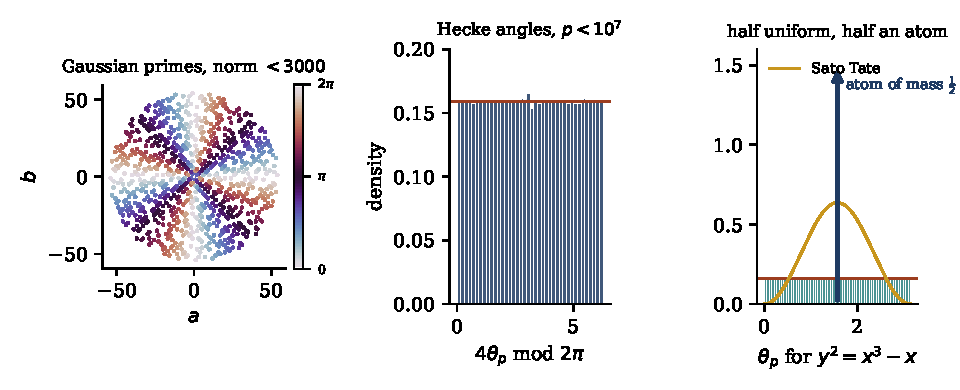
\includegraphics[width=\textwidth]{figs/gl1_hecke.pdf}
\caption{Left: the Gaussian primes of norm below $3000$ with their four associates, coloured by the Hecke angle $4\theta_p$. Middle: the angles $4\theta_p$ of the Gaussian primes below $10^7$ against the uniform law. Right: the Frobenius angles $\theta_p$ of $y^2=x^3-x$, uniform on $[0,\pi]$ for the split primes and equal to $\pi/2$ for the inert primes, against the Sato Tate density of a curve without complex multiplication.}\label{fig:gl1hecke}
\end{figure}

Hecke's theorem is Chebotarev's theorem for an infinite extension: the characters $\lambda_k$ do not factor through any finite Galois group, and the ``Galois group'' in which the Frobenius elements equidistribute is the circle, the connected component of the Sato Tate group of Section~\ref{sec:gl1cm}. The Gamma process of Theorem~\ref{thm:recipgammaproc} applies to the random integer coloured by $4\theta_p$ with $Y$ the circle and $\mu$ uniform, so that for a continuous $Q\ge0$ on the circle the Frobenius functional $\Xi_\sigma(Q)=(\sigma-1)\sum_{p\equiv1}e_p\log p\,Q(4\theta_p)$ converges to a GGC with Thorin measure $\frac12$ times the image of the uniform law under $1/Q$, the factor $\frac12$ being the density of the split primes, and the labelled factorisation converges to a Dirichlet process whose base measure is $\frac12$ times the uniform probability on the circle. The Mertens constants are given by Theorem~\ref{thm:pdmertensL} with the $L(1,\lambda_k)$ in place of the $L(1,\chi)$: for a trigonometric polynomial $Q(y)=\sum_{|k|\le m}c_ke^{iky}$, $\sum_{p\le x,\,p\equiv1}Q(4\theta_p)p^{-1}=\frac12c_0\log\log x+M(Q)+o(1)$ with $M(Q)=\frac12c_0M(4,1)+\frac12\sum_{0<|k|\le m}c_kS(\lambda_k)$, $S(\lambda_k)=\log L(1,\lambda_k)-\sum_{j\ge2}\sum_{\mathfrak p}\lambda_k(\mathfrak p)^j(jN\mathfrak p^j)^{-1}$; for the indicator of an arc the Fourier series of $M$ converges only conditionally and is better handled by smoothing.

\section{Complex multiplication}\label{sec:gl1cm}

Let $E$ be the curve $y^2=x^3-x$, of conductor $32$, with the automorphism $(x,y)\mapsto(-x,iy)$ giving complex multiplication by $\Z[i]$. Let $\psi$ be the Hecke character of $K=\Q(i)$ of conductor $\mathfrak f=(2+2i)$ with $\psi((\alpha))=\alpha$ for $\alpha\equiv1$ modulo $\mathfrak f$; it is well defined because $1$ is the only unit congruent to $1$ modulo $\mathfrak f$, and its infinity type is the identity. At the inert prime $(p)$, $p\equiv3$ modulo $4$, the primary generator is $-p$, since $4\in\mathfrak f$, so $\psi((p))=-p$.

\begin{theorem}[Deuring \cite{deuring1953}]\label{thm:gl1deuring}
$L(E,s)=L(s,\psi)$. Explicitly, for $p\equiv1$ modulo $4$ with primary $\pi=a+bi$, $a_p(E)=\pi+\bar\pi=2a$; for $p\equiv3$, $a_p(E)=0$; and the Euler factor at $p\equiv3$ is $(1+p^{1-2s})^{-1}$ on both sides.
\end{theorem}

The identity $a_p=2a$ with the primary normalisation was checked for all $332180$ primes $p\equiv1$ modulo $4$ below $10^7$ against the point counts of PARI; it holds without exception, and the other associates $-\pi$, $i\pi$, $-i\pi$ fail at every prime. The general theorem is that for $E/\Q$ with complex multiplication by an imaginary quadratic $K$, $L(E,s)=L(s,\psi)$ for a Hecke character $\psi$ of $K$ of infinity type the identity and conductor $\mathfrak f$ with $N_E=|d_K|N\mathfrak f$; here $32=4\cdot8$.

Deuring's theorem is reciprocity for $\GL_2$ reduced to $\GL_1$: the two dimensional representation $\rho_E$ of $\Gal(\overline\Q/\Q)$ is induced from the one dimensional representation $\psi$ of $\Gal(\overline\Q/K)$, which is abelian, so that $\rho_E$ is \emph{dihedral}, and its automorphic partner is the automorphic induction of $\psi$, the theta series $\sum_{\mathfrak a}\psi(\mathfrak a)q^{N\mathfrak a}$, a weight two form of level $32$ (Hecke). In the language of Chapter~\ref{ch:recip}, reciprocity for $E$ is the almost sure equality of $p\mapsto a_p(E)$ and $p\mapsto\pi+\bar\pi$, which Theorem~\ref{thm:gl1deuring} proves prime by prime.

\begin{proposition}[the angle law of a CM curve]\label{prop:gl1angle}
Write $a_p(E)=2\sqrt p\cos\theta_p$ with $\theta_p\in[0,\pi]$. Then $\theta_p$ is the angle of Section~\ref{sec:gl1hecke} for split $p$ and $\theta_p=\pi/2$ for inert $p$, and the law of $\theta_p$ is $\frac12\,\mathrm{Unif}[0,\pi]+\frac12\delta_{\pi/2}$. The moments are $\E\cos^2\theta_p=\frac14$ and $\E\cos^4\theta_p=\frac3{16}$, against $\frac14$ and $\frac18$ for the Sato Tate law; below $10^7$ the sample values are $0.24988$ and $0.18738$.
\end{proposition}

\begin{proof}
For split $p$, $\cos\theta_p=a/\sqrt p=\cos\arg\pi$ by Theorem~\ref{thm:gl1deuring}, and $|\arg\pi|$ is uniform on $[0,\pi]$ by the second part of Theorem~\ref{thm:gl1hecke}. The two classes have density $\frac12$ each by Dirichlet.
\end{proof}

The law in Proposition~\ref{prop:gl1angle} is the law of the trace of a Haar distributed element of the normaliser $N(\mathrm{U}(1))$ of the maximal torus $\mathrm{U}(1)$ in $\SU(2)$: the identity component contributes the uniform angle, the other component consists of matrices of trace zero. This is the Sato Tate group of a CM curve, and Chapter~\ref{ch:12} identifies it from the moments.

Now take the Rankin Selberg subordinator $X_\sigma$ of Section~\ref{sec:recipgalois}, with Laplace transform $D^S(\sigma+\lambda)/D^S(\sigma)$, $D^S(s)=L^S(s,\rho\otimes\check\rho)$, built over $\Q$, and the same subordinator $X^K_\sigma$ built over $K$ from the restriction of $\rho$ to $\Gal(\overline\Q/K)$, with $D^S_K(s)=L^S_K(s,\rho|_K\otimes\check\rho|_K)$ an Euler product over the primes of $K$.

\begin{theorem}[complex multiplication doubles the Gamma shape; this book]\label{thm:gl1cmshape}
Let $E/\Q$ be an elliptic curve, $\rho$ its normalised $\ell$ adic representation, $K$ an imaginary quadratic field and $\chi_K$ its character.
\begin{enumerate}
\item[(i)] $D^S_K(s)=D^S(s)\,L^S(s,\rho\otimes\check\rho\otimes\chi_K)$, the partial products being over the primes not dividing $N_E d_K$.
\item[(ii)] If $E$ has complex multiplication by $K$ then $D^S_K(s)=D^S(s)^2$ exactly, so that $X^K_\sigma$ has the law of the sum of two independent copies of $X_\sigma$ for every $\sigma>1$, and $(\sigma-1)X^K_\sigma$ converges to the Gamma law of shape $2$.
\item[(iii)] If $E$ has no complex multiplication by $K$ then $(\sigma-1)X^K_\sigma$ converges to the standard exponential law, the Gamma shape being $1$.
\end{enumerate}
\end{theorem}

\begin{proof}
(i) Restriction followed by induction multiplies by the regular representation of $\Gal(K/\Q)$: $\operatorname{Ind}_K^\Q\operatorname{Res}_K(\rho\otimes\check\rho)=(\rho\otimes\check\rho)\otimes(\mathsf 1\oplus\chi_K)$, and the $L$ function of an induced representation is the $L$ function over the smaller field of the representation induced from. At the level of Euler factors this is the statement that a prime $p$ of $\Q$ split in $K$ contributes two identical factors over $K$, while an inert $p$ contributes one factor at $p^2$, which equals the product of the factors of $\rho\otimes\check\rho$ and $\rho\otimes\check\rho\otimes\chi_K$ at $p$.

(ii) If $E$ has complex multiplication by $K$ then $a_p=0$ for every inert $p$, so $\tr\rho(\Frob_p)\chi_K(p)=\tr\rho(\Frob_p)$ for all $p\nmid N_Ed_K$, and $\rho\otimes\chi_K\cong\rho$ by Brauer and Nesbitt, both being semisimple. Hence $\rho\otimes\check\rho\otimes\chi_K\cong\rho\otimes\check\rho$, the two factors in (i) coincide, and $D_K^S=(D^S)^2$. A squared Laplace transform is the transform of a sum of two independent copies. By Theorem~\ref{thm:recipgamma} and its proof, which use only the order of the pole of $D^S$ at $s=1$, the Gamma shape is twice the shape over $\Q$, which is $1$ because $\rho$ is irreducible.

(iii) Over $K$ the Gamma shape is the order of the pole of $D^S_K$ at $1$, which by (i) is $1+m$, $m$ the order of the pole of $L(s,\rho\otimes\check\rho\otimes\chi_K)$. By modularity and the theory of Rankin and Selberg, $L(s,\rho\otimes\check\rho\otimes\chi_K)=L(s,f\times(f\otimes\chi_K))$ for the newform $f$ of $E$, and this has a pole at $s=1$ if and only if $f\otimes\chi_K=f$, that is $\rho\otimes\chi_K\cong\rho$, which forces $a_p=0$ for all inert $p$ of $K$, a set of density $\frac12$. For a curve without complex multiplication the primes with $a_p=0$ have density zero (Serre), and for a curve with complex multiplication by a field $K'\ne K$ they are, up to finitely many, the primes inert in $K'$, which exclude the primes split in $K'$ and inert in $K$, a set of density $\frac14$. So $f\otimes\chi_K=f$ forces complex multiplication by $K$, hence $m=0$ and the shape is $1$.
\end{proof}

For the curve $y^2=x^3-x$ the Laplace transforms were computed exactly from $D^S(s)=\zeta^{(2)}(s)L(s+1,\Sym^2E)$, the symmetric square from PARI, whose Euler factor at $2$ is trivial; this identity is the decomposition $\rho\otimes\check\rho=\mathsf 1\oplus\chi_4\oplus\operatorname{Ind}\tilde\psi^2$ together with $\Sym^2\rho=\operatorname{Ind}\tilde\psi^2\oplus\chi_4$. At $\sigma=1.001$ the transform of $(\sigma-1)X_\sigma$ at $\lambda=\frac12,1,2,4,8$ is $0.6672$, $0.5009$, $0.3345$, $0.2014$, $0.1127$ against $(1+\lambda)^{-1}=0.6667$, $0.5$, $0.3333$, $0.2$, $0.1111$, and over $K$ the squares $0.4452$, $0.2509$, $0.1119$, $0.0406$, $0.0127$ against $(1+\lambda)^{-2}$. The approach is at the rate $\sigma-1$ of the Euler Kronecker drift (Theorem~\ref{thm:recipdrift}): the deviations at $\lambda=1$ are $0.0810$, $0.0086$ and $0.0009$ at $\sigma-1=10^{-1},10^{-2},10^{-3}$ (Figure~\ref{fig:gl1cm}, left).

\begin{figure}[t]
\centering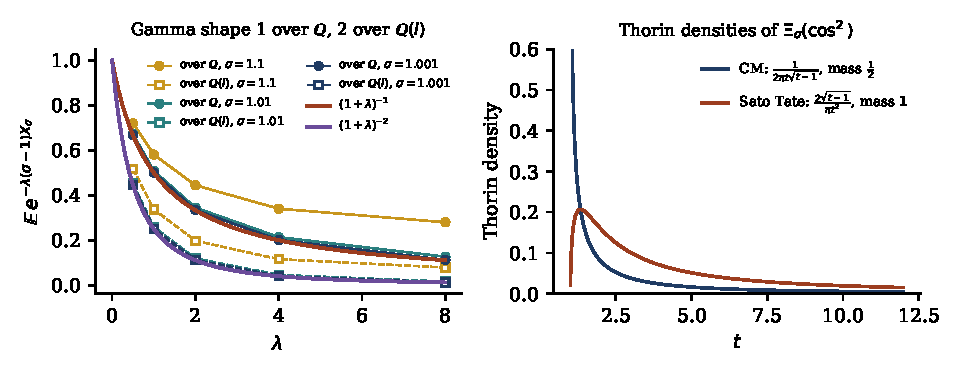
\includegraphics[width=\textwidth]{figs/gl1_cm.pdf}
\caption{Complex multiplication doubles the Gamma shape. Left: the Laplace transforms of $(\sigma-1)X_\sigma$ for $y^2=x^3-x$ over $\Q$ and over $\Q(i)$ at three values of $\sigma$, against the exponential and the Gamma$(2)$ limits of Theorem~\ref{thm:gl1cmshape}. Right: the Thorin densities of the limiting Frobenius functional $\Xi_\sigma(\cos^2)$ for a CM curve, the arcsine density of mass $\frac12$, and for a curve without complex multiplication, the image of the Sato Tate law, of mass $1$.}\label{fig:gl1cm}
\end{figure}

Theorem~\ref{thm:gl1cmshape} says what the Gamma shape of Chapter~\ref{ch:recip} measures when the base field changes: it counts the irreducible constituents with multiplicity, and restriction to $K$ splits $\rho$ exactly when $\rho$ is induced from $K$. For a CM curve the restriction is $\tilde\psi\oplus\tilde\psi^c$, two distinct characters, and the shape is $1^2+1^2=2$; a curve without complex multiplication by $K$ stays irreducible over $K$ and keeps shape $1$. The test is unconditional because both pole orders are theorems.

Finally the Frobenius functionals. Colour the prime factors of $N_\sigma$ by $y_p=4\theta_p$ on the circle for split $p$ and by a point $\{\mathrm{in}\}$ for inert $p$, so $Y=S^1\sqcup\{\mathrm{in}\}$ with $\mu=\frac12\mathrm{Unif}+\frac12\delta_{\mathrm{in}}$. Theorem~\ref{thm:recipggcfun} gives, for continuous $Q\ge0$ on $Y$, the GGC limit of $\Xi_\sigma(Q)$ with Thorin measure the image of $\mu$ under $1/Q$ on $\{Q>0\}$. Two cases are instructive. For $Q=\mathsf 1_{\mathrm{in}}$ the limit is the Gamma law of shape $\frac12$, with Thorin measure $\frac12\delta_1$, and the atom at zero $e^{-h_3(1)}(\sigma-1)^{1/2}$ is the Landau phenomenon of Theorem~\ref{thm:gl1landau}. For $Q=\cos^2\theta_p=a^2/p$, a quarter of the squared normalised trace, the limit has Thorin measure $\frac12$ times the image of the uniform law on $[0,\pi]$ under $\theta\mapsto1/\cos^2\theta$, that is the measure $\frac{dt}{2\pi t\sqrt{t-1}}$ on $(1,\infty)$, of total mass $\frac12$ (Figure~\ref{fig:gl1cm}, right): the Frobenius functional $\Xi_\sigma(\cos^2)$ of a CM curve is asymptotically a GGC with an explicit arcsine Thorin density. For a curve without complex multiplication the same functional has the Thorin density $\frac{2}{\pi t^2}\sqrt{t-1}$ of total mass one on $(1,\infty)$, the image of the Sato Tate law.

\section{The Thorin measure of a degree one \texorpdfstring{$L$}{L} function}\label{sec:gl1thorin}

Let $\chi$ be a primitive real character modulo $q$ and $\kappa\in\{0,1\}$ its parity, so that the completed function $\Lambda(s,\chi)=(q/\pi)^{s/2}\Gamma(\frac{s+\kappa}2)L(s,\chi)$ satisfies $\Lambda(s,\chi)=\Lambda(1-s,\chi)$ with root number $+1$. Put $\Xi_\chi(w)=\Lambda(\frac12+w,\chi)$, an even entire function of order one, and write its zeros as $\pm i\gamma_k$, with multiplicity, choosing one $\gamma_k$ from each pair; only $\gamma_k^2$ enters below.

\begin{theorem}[Thorin form in degree one]\label{thm:gl1thorin}
Suppose $L(\frac12,\chi)\ne0$. Then $\Xi_\chi(\sqrt\lambda)/\Xi_\chi(0)=\prod_k(1+\lambda/\gamma_k^2)$ for $\lambda\ge0$, the product converging absolutely, and GRH for $\chi$ holds if and only if $\Xi_\chi(0)/\Xi_\chi(\sqrt\lambda)$ is the Laplace transform of a GGC, in which case the Thorin measure is $\sum_k\delta_{\gamma_k^2}$ and the GGC is $\sum_kE_k/\gamma_k^2$ with $E_k$ independent standard exponentials. For every basepoint $\frac12+a$ with $a\ge\frac12$ the shifted representation of Theorem~\ref{thm:10dshift} holds unconditionally, with the Thorin density $V_a$ positive.
\end{theorem}

\begin{proof}
This is Theorem~\ref{thm:10bmain} for $n=1$, which Section~\ref{sec:10bcompletion} admits; the proof reads: $\Xi_\chi$ is even and entire of order one, so Hadamard's product has the form $e^{bw}\prod(1+w^2/\gamma_k^2)$ with $b=0$ by evenness, and $\Xi_\chi(0)\ne0$ by hypothesis. The nonvanishing hypothesis holds for $\chi_4$, where $L(\frac12,\chi_4)=0.6677$, and is Chowla's conjecture for real $\chi$ in general; a zero of order $2m$ at $w=0$ is removed by dividing by $w^{2m}$ and changes nothing else. The last assertion is Theorem~\ref{thm:10dshift}(iii).
\end{proof}

For $\chi_4$ the first zeros are at $\gamma=6.020949$, $10.243770$, $12.988098$, $16.342607$, $18.291993$, and there are $3130$ below height $3000$, where the counting function $\frac T{2\pi}\log\frac{4T}{2\pi e}$ predicts $3129.7$. With these zeros and the tail $\int_T^\infty\log(1+\lambda/t^2)\,dN(t)$ from the smooth counting function, the product $\prod_k(1+\lambda/\gamma_k^2)$ agrees with $\Xi_{\chi_4}(\sqrt\lambda)/\Xi_{\chi_4}(0)$ to relative error $2\cdot10^{-8}$ at $\lambda=1$, $3\cdot10^{-7}$ at $\lambda=16$, $2\cdot10^{-6}$ at $\lambda=100$ and $9\cdot10^{-6}$ at $\lambda=400$, where the ratio is $2.8\cdot10^7$; the residual error is the tail approximation, which grows with $\lambda$ (Figure~\ref{fig:gl1zeros}, left). The right panel of the figure shows the Thorin density of Theorem~\ref{thm:10dshift} at three basepoints $\frac12+a$: by Theorem~\ref{thm:lapcauchy} it is the measure $\sum_k\delta_{\gamma_k}$ on the $\sqrt z$ axis smoothed by Cauchy noise of scale $a$, and as $a\downarrow0$ the peaks sharpen into the atoms $\delta_{\gamma_k^2}$ of Theorem~\ref{thm:gl1thorin}.

\begin{figure}[t]
\centering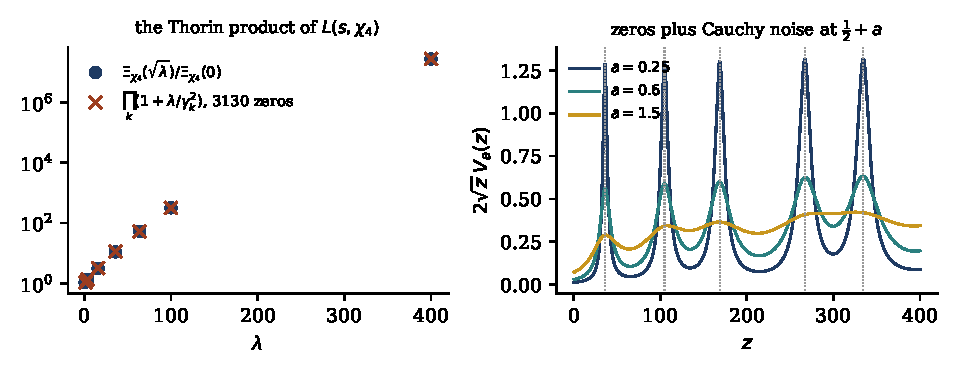
\includegraphics[width=\textwidth]{figs/gl1_zeros.pdf}
\caption{The Thorin measure of $L(s,\chi_4)$. Left: $\Xi_{\chi_4}(\sqrt\lambda)/\Xi_{\chi_4}(0)$ against the product over the $3130$ zeros below height $3000$ with the tail correction; the two agree to between $2\cdot10^{-8}$ and $9\cdot10^{-6}$. Right: the shifted Thorin density $V_a(z)$ of Theorem~\ref{thm:10dshift}, drawn as $2\sqrt zV_a(z)=\frac1\pi\sum_k\bigl[\frac{a}{a^2+(\sqrt z-\gamma_k)^2}+\frac{a}{a^2+(\sqrt z+\gamma_k)^2}\bigr]$, for $a=0.25$, $0.6$ and $1.5$; the vertical lines mark $\gamma_k^2$ for the first five zeros.}\label{fig:gl1zeros}
\end{figure}

The Galois face is different in degree one from degree two, and the difference is worth recording. The sine squared lemma (Lemma~\ref{lem:10dsin2}) represents $f(\alpha)/f(\alpha+\sqrt\lambda)$ through a GGC when $\log f(\alpha+s)$ is the Laplace transform of a positive measure, as it is for $\zeta$, for $\zeta_K$, and for every Rankin Selberg $L$ function. For $L(s,\chi)$ with $\chi$ real the logarithmic coefficients $\chi(p)^k\log p/k$ change sign, and the formula of the lemma produces a signed density: for small $z$ it is $-\frac{\sqrt z}{4\pi}(\log L)'''(\alpha)=\frac{\sqrt z}{4\pi}\sum_n\Lambda_\chi(n)(\log n)^2n^{-\alpha}$, which for $\chi_4$ equals $-0.257$, $-0.156$, $-0.090$ at $\alpha=1.1,1.5,2$, whereas for $\zeta_{\Q(i)}=\zeta L(\cdot,\chi_4)$ the same quantity is $2000$, $15.8$, $1.86$. So on the Galois face a real character is not by itself a GGC object; its Dedekind zeta function is, and so is its completed $L$ function at every basepoint $\alpha\ge1$ by Theorem~\ref{thm:gl1thorin}, the gamma factor supplying the positivity that the Euler product lacks. This is the degree one instance of the remark in Chapter~\ref{ch:lap} that the two faces carry the same measure but not the same positivity.

\section{What this adds to the programme}

The chapter proves, in degree one, the three things that the rest of the book conjectures or assumes in degree two: equidistribution with the right base measure (Dirichlet, Hecke), reciprocity (Kronecker Weber, Artin, Deuring), and the Thorin structure at every basepoint to the right of the zeros. Two of its theorems are new in substance. Theorem~\ref{thm:gl1landau}, whose constant is a standard application of Landau and Wirsing, identifies the Wirsing constant of the atom at zero of Chapter~\ref{ch:pd} with Landau's constant, corrected by the probability $\prod_{p\equiv3}(1-p^{-2})$ of squarefreeness in the class, and locates Landau's theorem inside the Dirichlet process. Theorem~\ref{thm:gl1cmshape} shows that the Gamma shape of Theorem~\ref{thm:recipgamma}, which detects irreducibility over $\Q$, detects complex multiplication when the base field is changed, with an exact identity $D_K^S=(D^S)^2$ rather than an asymptotic one. It also shows what the Gamma shape cannot do: over $\Q$ a CM curve and a non CM curve both have shape $1$, and the difference between them is visible only in the Thorin measure of the Frobenius functionals (an arcsine density of mass $\frac12$ against a Sato Tate density of mass $1$) or after base change.

\section{Notes}

The theorem of Kronecker and Weber, Artin's reciprocity law and Hecke's Gr\"ossencharaktere are in any account of class field theory; Neukirch \cite{neukirch1999} is the reference used here, and Tate's thesis \cite{tate1950} is the adelic form of Theorem~\ref{thm:gl1cft}(iii). Hecke's equidistribution theorem is \cite{hecke1920}; its discrepancy under GRH is treated by Kubilius \cite{kubilius1955}. Mertens' theorem for progressions is due to Williams \cite{williams1974}. Landau's theorem on sums of two squares is \cite{landau1908}; the constant is often attributed jointly to Ramanujan, and Wirsing's theorem \cite{wirsing1961} is the general form. Deuring's theorem is \cite{deuring1953}; Silverman's second volume \cite{silverman1994} gives the proof and the computation of the Hecke character of $y^2=x^3-x$, and Ireland and Rosen \cite{irelandrosen1990} the elementary count $a_p=2a$ with the primary normalisation. The Rankin Selberg criterion for $f\otimes\chi=f$ used in Theorem~\ref{thm:gl1cmshape} is in \cite{iwanieckowalski2004}. Theorem~\ref{thm:gl1dirichlet}(iii) is Williams' theorem, and (i) and (ii) are its Dirichlet process reading; Theorem~\ref{thm:gl1landau} is classical apart from the identification with $h_3(1)$; Theorems~\ref{thm:gl1cmshape} and \ref{thm:gl1thorin} are new as formulated. Their ingredients are the theorems cited and Chapters~\ref{ch:10b}, \ref{ch:recip} and \ref{ch:pd}.

\section{Exercises}

\begin{enumerate}
\item Show that among the four associates $\pm\pi,\pm i\pi$ of a Gaussian prime exactly two, $\pi$ and $-\pi$, have odd real part, and that $a_p=2\operatorname{Re}\pi$ holds for the primary one only. Determine the proportion of primes at which the normalisation $a\equiv1$ modulo $4$ alone gives the right sign.
\item Compute $M(8,a)$ for the four classes modulo $8$ from $L(1,\chi)$ for the three nonprincipal characters, and check against the primes below $10^7$.
\item Show that the number of $n\le x$ all of whose prime factors are congruent to $1$ modulo $q$ is asymptotic to $c_qx(\log x)^{1/\varphi(q)-1}$, and express $c_q$ through the $L(1,\chi)$.
\item For $E$ with complex multiplication by $K$, show that the Sato Tate group is $N(\mathrm{U}(1))$ and that the moments of $\cos\theta_p$ are $\E\cos^{2m}\theta_p=\frac12\binom{2m}m4^{-m}$. Verify the values $\frac14$ and $\frac3{16}$.
\item Show that for $Q=\cos^2(y/4)$ on the circle the image of the uniform law under $1/Q$ has density $1/(\pi t\sqrt{t-1})$ on $(1,\infty)$, and that the corresponding GGC has Laplace transform $\exp(-\frac12\int_1^\infty\log(1+\lambda/t)\frac{dt}{\pi t\sqrt{t-1}})$. Compute this integral in closed form.
\item Prove Theorem~\ref{thm:gl1cmshape}(i) at the level of Euler factors for a split and for an inert prime.
\item Let $\chi$ be a real character with $L(\frac12,\chi)=0$ of order $2m$. Show that $\Xi_\chi(\sqrt\lambda)/(\lambda^m\Xi_\chi^{(2m)}(0)/(2m)!)$ is again $\prod(1+\lambda/\gamma_k^2)$ over the remaining zeros.
\end{enumerate}

\section{Open problems}

\begin{problem}[the discrepancy of Hecke angles]\label{op:gl1disc}
For the Gaussian primes below $x$ the discrepancy of $4\theta_p$ satisfies $\sqrt{\pi_1(x)}D=1.07$ at $x=10^6$ and $0.84$ at $x=10^7$. Determine whether $\sqrt{\pi_1(x)}D$ has a limit law as $x\to\infty$ (the Kolmogorov law would be the Brownian bridge prediction, as in Open Problem~\ref{op:disc} for Sato Tate), or whether the arithmetic of the $L(s,\lambda_k)$ forces a different law; the same question for the imaginary quadratic fields of class number one.
\end{problem}

\begin{problem}[Euler Kronecker constants of Hecke characters]\label{op:gl1rate}
The rate of convergence of the Dirichlet process of Section~\ref{sec:gl1hecke} is governed, for the means, by the constants $L'/L(1,\lambda_k)$ in the same way that Theorem~\ref{thm:recipdrift} is governed by Euler Kronecker constants. Compute these constants for $\Q(i)$ and $k\le20$, determine the sign pattern of the deficits of the arcs, and find the analogue of Theorem~\ref{thm:pdrate} for the circle, where no arc is a finite union of classes.
\end{problem}

\begin{problem}[an effective Gamma shape test]\label{op:gl1cm}
Theorem~\ref{thm:gl1cmshape} distinguishes complex multiplication by $K$ through a limit as $\sigma\downarrow1$. By Faltings' theorem finitely many $a_p$ determine $\rho$ up to isomorphism, so finitely many primes decide whether $\rho\otimes\chi_K\cong\rho$. Find an explicit bound, in terms of $N_E$ and $d_K$, on the primes needed so that the empirical Laplace transform of $(\sigma-1)X^K_\sigma$ at a suitable $\sigma$ separates shape $1$ from shape $2$ with a proof, and compare with the bound from the effective Chebotarev theorem.
\end{problem}

\begin{compproblem}[class number one fields]\label{cp:gl1}
Objective: for each of the nine imaginary quadratic fields of class number one, compute the Hecke angles of the split primes below $10^9$, their discrepancy, and the Mertens constants of the arcs of length $\pi/2$, with the predicted constants from $L(1,\lambda_k)$. For the CM curves of conductor $27$, $32$, $36$, $49$, $121$ and $256$ verify Theorem~\ref{thm:gl1cmshape}(ii) from the exact Laplace transforms at $\sigma=1.0001$. Starting point: \texttt{g1.py}, \texttt{g3.py} and \texttt{g4.py}.
\end{compproblem}
